\documentclass[11pt,a4paper]{article}
\usepackage[margin=2.5cm]{geometry}
\usepackage{amsmath,amssymb}
\usepackage{tikz}
\setlength{\emergencystretch}{4em}

% --- notation shared by both parts -------------------------------------------------
\newcommand{\vt}{\vartheta}                    % conservative entropic variable
\newcommand{\hth}{{h_{\vartheta}}}               % dh/dtheta at fixed (P,q)  (conjugate variable)
\newcommand{\hq}{{h_q}}                          % dh/dq at fixed (P,theta)  (modified chemical potential)
\newcommand{\bu}{\mathbf{u}}
\newcommand{\bn}{\mathbf{n}}
\newcommand{\ez}{\hat{\mathbf{z}}}
\newcommand{\bJ}{\mathbf{J}}
\newcommand{\bF}{\mathbf{F}}
\newcommand{\bnabla}{\boldsymbol{\nabla}}
\newcommand{\btau}{\boldsymbol{\tau}}
\newcommand{\bomega}{\boldsymbol{\omega}}
\newcommand{\pdc}[3]{\left.\frac{\partial #1}{\partial #2}\right|_{#3}}
\newcommand{\code}[1]{\texttt{#1}}
% discrete operators (Part II): difference and average along x or z
\newcommand{\dx}{\delta_x}
\newcommand{\dz}{\delta_z}
\newcommand{\Ix}{\mathcal{I}_x}
\newcommand{\Iz}{\mathcal{I}_z}
\newcommand{\Ixz}{\mathcal{I}_{xz}}

\title{Energy-consistent anelastic and compressible box models:\\ continuous equations and numerical scheme}
\author{Notes on the \code{TraceableEnergetics} code (AN2D and FC2D)}
\date{}

\begin{document}
\maketitle
\tableofcontents

\bigskip
\noindent\textbf{Conventions.}
AN2D denotes the 2D anelastic model and FC2D the 2D fully compressible box model. Part~I contains only continuous physics;
Part~II specifies the discrete scheme completely enough to be re-implemented, and derives its conservation properties.
Where this document and any other write-up disagree, it follows the code. The correspondence between mathematical symbols and code names is given in Table~\ref{tab:symbols}.

% =====================================================================================
\part{Continuous physics}
% =====================================================================================

\section{Setting and variables}
Both models are posed in a vertical box $(x,z)\in[0,L_x]\times[0,L_z]$ with $z$ upward and no dependence on $y$.
The velocity is $\bu=(u,w)$ and $\bomega=\omega\,\hat{\mathbf y}$ with
\begin{equation}
  \omega = \partial_z u - \partial_x w .
\end{equation}
Gravity acts along $-\ez$ with constant magnitude $g>0$. The geopotential is
\begin{equation}
  \Phi(z) = g\,(z - z_0),\qquad \bnabla\Phi = g\,\ez ,
\end{equation}
with $z$ the height above the bottom of the box and $z_0$ the height at which $\Phi$ vanishes (\code{space.z0}, by default the bottom, $z_0=0$). The origin of $\Phi$ is arbitrary: shifting it changes the total energy by a constant times the (conserved) mass.

The fluid is a binary mixture (solvent and solute) with mass fraction $q$ of solute and an entropic
variable $\vt$ that is a function of the specific entropy $s$ and of $q$ only, $\vt=\vt(s,q)$, and is therefore
conserved by adiabatic, isohaline motion. In the experiments $\vt$ is the potential temperature; any entropic variable is allowed
(e.g.\ $\vt=s$).

\begin{table}[ht]
\centering\small
\begin{tabular}{p{4.3cm}p{6.0cm}p{4.9cm}}
\hline
Symbol & Meaning [unit] & Code \\ \hline
$L_x,L_z,g$ & box size [m], gravity [m\,s$^{-2}$] & \code{space.Lx}, \code{space.Lz}, \code{space.g} \\
$z_0$ & height above the bottom where $\Phi=0$ [m] & \code{space.z0} \\
$\rho$, $v=1/\rho$ & density [kg\,m$^{-3}$], specific volume & \code{m[:,:,1]} (FC2D) \\
$P$ & pressure [Pa] & \code{p} \\
$p$ & reduced pressure (AN2D), $p=(P-P_R)/\rho_R$ [J\,kg$^{-1}$] & \code{scratch.phi} \\
$\vt$, $q$ & entropic variable, solute fraction [kg\,kg$^{-1}$] & \code{consvar}, \code{q} \\
$h(P,\vt,q)$ & specific enthalpy [J\,kg$^{-1}$] & \code{specific\_enthalpy} \\
$h_\vt=\partial h/\partial\vt|_{P,q}$ & conjugate variable of $\vt$ & \code{conjvar} \\
$h_q=\partial h/\partial q|_{P,\vt}$ & modified chemical potential [J\,kg$^{-1}$] & \code{chempot} \\
$\mu=\partial h/\partial q|_{P,s}$ & chemical potential [J\,kg$^{-1}$] & (enters only through $\Gamma$) \\
$T$ & temperature [K] & \code{T} \\
$c_p$ & heat capacity [J\,kg$^{-1}$K$^{-1}$] & \code{Cp} \\
$B=h-\vt h_\vt-q h_q$ & Bernoulli potential [J\,kg$^{-1}$] & \code{B} \\
$b$ & buoyancy (AN2D) [m\,s$^{-2}$] & \code{buoyancy} \\
$K=|\bu|^2/2$ & kinetic energy per unit mass & \code{K} \\
$\btau$, $\eta$ & viscous stress, dynamic viscosity [Pa\,s] & \code{dyn\_visc} \\
$\kappa_T,\kappa_q$ & diffusivities [m$^2$\,s$^{-1}$] & \code{k\_T}, \code{k\_q} \\
$\Gamma$ & barodiffusion coefficient [Pa$^{-1}$] & \code{Gamma} \\
$\partial\mu/\partial P|_{T,q}$, $\partial\mu/\partial q|_{P,T}$ & derivatives defining $\Gamma$ & \code{chemical\_potential\_derivatives} \\
$\partial\vt/\partial q|_{P,T}$ & used in the flux of $\vt$ & \code{dcons\_dq} \\
$\bJ_\vt,\bJ_q$ & diffusive fluxes of $\vt$, $q$ & \code{consflux}, \code{qflux} \\
$\sigma_\vt$ & production of $\rho\vt$ & \code{sigma\_cons} \\
$\rho\varepsilon$ & viscous dissipation per unit volume & \code{rho\_eps} \\
$\rho_R(z),P_R(z)$ & anelastic reference density, pressure & \code{rho\_R}, \code{p\_R} \\
\hline
\end{tabular}
\caption{Mathematical symbols and code names (Greek letters in the source are spelled out). The capital $P$ is the full pressure; $p$ is the reduced pressure of the anelastic model.
The fluid (equation of state) is supplied by the \code{ClimFluids} library; AN2D is the package \code{CFAnelastics} and FC2D the package \code{CFCompressible}. The flux laws of \S\ref{sec:irr} are the functions \code{salt\_flux}, \code{heat\_to\_consvar} and \code{consvar\_flux}, and the schemes $\kappa_T,\kappa_q,\eta$ the types \code{ThermoFluxConsistent}, \code{ThermoFluxDowngradient} and \code{ViscosityScheme}, all of \code{CFDiffusionSchemes}.}
\label{tab:symbols}
\end{table}

\section{Thermodynamics}\label{sec:thermo}
\subsection{Fundamental relation}
The fluid is specified by its specific enthalpy $h(P,\vt,q)$, with
\begin{equation}
  \mathrm{d}h = v\,\mathrm{d}P + \hth\,\mathrm{d}\vt + \hq\,\mathrm{d}q,\qquad
  \hth=\pdc{h}{\vt}{P,q},\quad \hq=\pdc{h}{q}{P,\vt},\quad v=\pdc{h}{P}{\vt,q}.
  \label{eq:dh}
\end{equation}
The internal energy is $e=h-Pv$. The Bernoulli potential is
\begin{equation}
  B = h-\vt\,\hth-q\,\hq .
  \label{eq:B}
\end{equation}
From \eqref{eq:dh}, $\mathrm{d}B = v\,\mathrm{d}P-\vt\,\mathrm{d}\hth-q\,\mathrm{d}\hq$, hence the pressure force can be
written without $\bnabla P$:
\begin{equation}
  -v\,\bnabla P = -\vt\,\bnabla\hth - q\,\bnabla\hq - \bnabla B .
  \label{eq:thermoforce}
\end{equation}
Also, for $\rho e=\rho h-P$ regarded as a function of $(\rho,\rho\vt,\rho q)$,
\begin{equation}
  \mathrm{d}(\rho e) = B\,\mathrm{d}\rho + \hth\,\mathrm{d}(\rho\vt) + \hq\,\mathrm{d}(\rho q).
  \label{eq:dpe}
\end{equation}
Indeed $\mathrm{d}(\rho h-P)=h\,\mathrm{d}\rho+\rho\,(v\,\mathrm{d}P+\hth\,\mathrm{d}\vt+\hq\,\mathrm{d}q)-\mathrm{d}P
=h\,\mathrm{d}\rho+\rho\hth\,\mathrm{d}\vt+\rho\hq\,\mathrm{d}q$ (using $\rho v=1$), and
$\rho\,\mathrm{d}\vt=\mathrm{d}(\rho\vt)-\vt\,\mathrm{d}\rho$, likewise for $q$. This is what makes $(\rho,\rho\vt,\rho q)$ the natural prognostic
variables for energy conservation.

\subsection{Temperature, entropy and chemical potential}
The temperature and entropy are defined by $\mathrm{d}h=T\,\mathrm{d}s+v\,\mathrm{d}P+\mu\,\mathrm{d}q$, i.e.\ $T=\partial h/\partial s|_{P,q}$ and $\mu=\partial h/\partial q|_{P,s}$.
Since $s=s(\vt,q)$ does not depend on $P$, comparing with \eqref{eq:dh} at fixed $P$ gives
\begin{equation}
  T\,\mathrm{d}s+\mu\,\mathrm{d}q=\hth\,\mathrm{d}\vt+\hq\,\mathrm{d}q
  \quad\Longrightarrow\quad
  s_\vt:=\pdc{s}{\vt}{q}=\frac{\hth}{T},\qquad s_q:=\pdc{s}{q}{\vt}=\frac{\hq-\mu}{T},
  \label{eq:sderiv}
\end{equation}
both functions of $(\vt,q)$ only. By the chain rule on $h(P,\vt(P,T,q),q)$,
\begin{equation}
  \pdc{h}{q}{P,T}=\hth\,\pdc{\vt}{q}{P,T}+\hq .
  \label{eq:hq}
\end{equation}
The Gibbs function $G=h-Ts$ satisfies $\mathrm{d}G=-s\,\mathrm{d}T+v\,\mathrm{d}P+\mu\,\mathrm{d}q$, hence the Maxwell relation
$\partial\mu/\partial T|_{P,q}=-\partial s/\partial q|_{P,T}$, and $\partial h/\partial q|_{P,T}=\mu+T\,\partial s/\partial q|_{P,T}$.

\subsection{Barodiffusion coefficient}
Write $\mu(P,T,q)$ for the chemical potential as a function of pressure, temperature and composition. The barodiffusion coefficient is
\begin{equation}
  \Gamma = -\frac{\partial\mu/\partial P}{\partial\mu/\partial q},
  \label{eq:Gamma}
\end{equation}
with the derivatives at fixed $(T,q)$ and fixed $(P,T)$ respectively. It is independent of the choice of entropic variable, as $\mu(P,T,q)$ is.
The heat flux below uses $\partial\vt/\partial q$ at fixed $(P,T)$; for $\vt$ equal to the potential temperature of the fluid in Appendix~\ref{app:eos} this derivative vanishes.

\subsection{Equation of state}
The equation of state is a general (nonlinear) binary fluid $h(P,\vt,q)$; Appendix~\ref{app:eos}
gives the explicit one currently used, with the constants left symbolic. Neither model assumes an ideal gas.
The models require from the fluid, as functions of $(P,\vt,q)$: $h$, $v$, $T$, $\hth$, $\hq$, $c_p$, $\partial_q\vt|_{P,T}$;
as functions of $(P,T,q)$: $\partial\mu/\partial P$ and $\partial\mu/\partial q$; and, for FC2D only, $P(v,\vt,q)$ and the sound speed $c$.
AN2D only evaluates thermodynamic functions at the reference pressure $P_R(z)$.

\section{Irreversible processes (common to both models)}\label{sec:irr}
\subsection{Viscous stress}
With constant dynamic viscosity $\eta$ and the Stokes hypothesis (zero bulk viscosity),
\begin{equation}
  \btau = 2\eta\Big(\mathsf S-\tfrac13(\bnabla\!\cdot\bu)\,\mathsf I\Big),\quad
  \mathsf S=\tfrac12\big(\bnabla\bu+\bnabla\bu^{\!\top}\big),\qquad
  \bF=\bnabla\!\cdot\btau = \eta\Big(\tfrac43\bnabla D + (\partial_z\omega,\,-\partial_x\omega)\Big),
  \label{eq:tau}
\end{equation}
where $D=\bnabla\!\cdot\bu$ and $\bF$ is the viscous force per unit volume [N\,m$^{-3}$]. (With $\partial_y=0$ and constant $\eta$,
$\bnabla\!\cdot\btau=\eta(\nabla^2\bu+\tfrac13\bnabla D)$ and $\nabla^2\bu=\bnabla D+(\partial_z\omega,-\partial_x\omega)$.) The viscous dissipation per unit volume is
\begin{equation}
  \rho\varepsilon = \btau:\bnabla\bu
  = \tfrac{2\eta}{3}\big(u_x^2+w_z^2+(u_x-w_z)^2\big)+\eta\,(u_z+w_x)^2\;\ge 0,
  \label{eq:diss}
\end{equation}
and satisfies $\rho\varepsilon=\bnabla\!\cdot(\bu\cdot\btau)-\bu\cdot\bF$.

\subsection{Heat and composition fluxes}
Let $\bJ_q$ be the diffusive flux of solute (so $\rho\,\mathrm{D}q/\mathrm{D}t=-\bnabla\!\cdot\bJ_q$) and $\bJ_Q$ the total heat flux. The model uses
the reduced heat flux $\bJ'_Q=\bJ_Q-\partial_qh|_{P,T}\,\bJ_q$ and the laws (no cross-diffusion)
\begin{align}
  \bJ_q &= -\rho_f\,\kappa_q\,\big(\bnabla q-\Gamma\,\bnabla P_f\big),\label{eq:Jq}\\
  \bJ'_Q &= -\rho_f\,c_p\,\kappa_T\,\bnabla T .\label{eq:JQ}
\end{align}
For FC2D, $\rho_f=\rho$ and $P_f=P$. For AN2D, $\rho_f=\rho_R$, $P_f=P_R$, and all thermodynamic quantities (including $\Gamma$) are evaluated at $P=P_R(z)$; the pressure gradient is then $\bnabla P_R=-\rho_Rg\,\ez=-\rho_R\bnabla\Phi$.
Note $\bnabla\mu|_T=\partial_P\mu\,\bnabla P+\partial_q\mu\,\bnabla q=\partial_q\mu\,(\bnabla q-\Gamma\bnabla P)$, so $\bJ_q=-(\rho_f\kappa_q/\partial_q\mu)\,\bnabla\mu|_T$.
An alternative ``down-gradient'' option, $\bJ_\vt=-\rho_f\kappa_T\bnabla\vt$, $\bJ_q=-\rho_f\kappa_q\bnabla q$, $\sigma_\vt=0$, exists for comparison; it is not energy-conserving.

\subsection{Evolution equation of $\vt$ and the production $\sigma_\vt$}\label{sec:sigma}
The enthalpy equation of a viscous binary fluid with heat flux $\bJ_Q$ is
\begin{equation}
  \rho\frac{\mathrm{D}h}{\mathrm{D}t}=\frac{\mathrm{D}P}{\mathrm{D}t}-\bnabla\!\cdot\bJ_Q+\rho\varepsilon .
\end{equation}
Substituting $\mathrm{D}h=v\,\mathrm{D}P+\hth\,\mathrm{D}\vt+\hq\,\mathrm{D}q$ from \eqref{eq:dh} and $\rho\,\mathrm{D}q/\mathrm{D}t=-\bnabla\!\cdot\bJ_q$:
\begin{equation}
  \rho\hth\frac{\mathrm{D}\vt}{\mathrm{D}t}=-\bnabla\!\cdot\bJ_Q+\hq\,\bnabla\!\cdot\bJ_q+\rho\varepsilon
  =-\bnabla\!\cdot\big(\bJ_Q-\hq\bJ_q\big)-\bJ_q\!\cdot\bnabla\hq+\rho\varepsilon .
\end{equation}
Define the flux of $\vt$ and use $\hth\,\bnabla\!\cdot\bJ_\vt=\bnabla\!\cdot(\hth\bJ_\vt)-\bJ_\vt\!\cdot\bnabla\hth$:
\begin{equation}
  \bJ_\vt=\frac{\bJ_Q-\hq\bJ_q}{\hth}=\frac{\bJ'_Q}{\hth}+\pdc{\vt}{q}{P,T}\bJ_q,\qquad
  \rho\frac{\mathrm{D}\vt}{\mathrm{D}t}=-\bnabla\!\cdot\bJ_\vt+\sigma_\vt,\qquad
  \hth\,\sigma_\vt=\rho\varepsilon-\bJ_\vt\!\cdot\bnabla\hth-\bJ_q\!\cdot\bnabla\hq .
  \label{eq:sigma}
\end{equation}
(The second form of $\bJ_\vt$ follows from \eqref{eq:hq}.) In conservative form, $\partial_t(\rho\vt)+\bnabla\!\cdot(\rho\vt\bu)=-\bnabla\!\cdot\bJ_\vt+\sigma_\vt$ given mass conservation. This is exactly the
system the models solve; it is also exactly energy-conserving (\S\ref{sec:conservation}). Note $\hth\bJ_\vt+\hq\bJ_q=\bJ_Q$: the energy flux carried by the diffusive fluxes is the total heat flux.

\subsection{Entropy production}\label{sec:entropy}
The second law fixes the sign of the \emph{entropy} production, not of $\sigma_\vt$. From $T\,\mathrm{d}s=\mathrm{d}h-v\,\mathrm{d}P-\mu\,\mathrm{d}q$ and the enthalpy equation,
\begin{equation}
  \rho T\frac{\mathrm{D}s}{\mathrm{D}t}=-\bnabla\!\cdot\bJ_Q+\mu\,\bnabla\!\cdot\bJ_q+\rho\varepsilon
  \quad\Longrightarrow\quad
  \rho\frac{\mathrm{D}s}{\mathrm{D}t}=-\bnabla\!\cdot\bJ_s+\sigma_s,\quad
  \bJ_s=\frac{\bJ_Q-\mu\bJ_q}{T},
\end{equation}
\begin{equation}
  T\sigma_s=\rho\varepsilon-\bJ_s\!\cdot\bnabla T-\bJ_q\!\cdot\bnabla\mu .
\end{equation}
(Expand $-\bnabla\!\cdot\bJ_Q/T+\mu\bnabla\!\cdot\bJ_q/T=-\bnabla\!\cdot\bJ_s-\bJ_s\!\cdot\bnabla T/T-\bJ_q\!\cdot\bnabla\mu/T$.)
With $\bJ_Q=\bJ'_Q+(\mu+T\partial_qs|_{P,T})\bJ_q$ one has $\bJ_s=\bJ'_Q/T+\partial_qs|_{P,T}\bJ_q$, and by the Maxwell relation
$\partial_qs|_{P,T}\,\bnabla T+\bnabla\mu=\bnabla\mu|_T$. Therefore
\begin{equation}
  T\sigma_s=\rho\varepsilon-\frac{\bJ'_Q\!\cdot\bnabla T}{T}-\bJ_q\!\cdot\bnabla\mu|_T
  =\rho\varepsilon+\rho\,c_p\kappa_T\frac{|\bnabla T|^2}{T}+\rho\kappa_q\,\partial_q\mu\,\big|\bnabla q-\Gamma\bnabla P_f\big|^2\;\ge 0,
  \label{eq:entropyprod}
\end{equation}
by \eqref{eq:diss}, \eqref{eq:Jq}, \eqref{eq:JQ} and $\partial_q\mu>0$ (for the fluid of the appendix $\partial_q\mu=R_sT/q$). Every term is non-negative.

\paragraph{Relation between $\sigma_\vt$ and $\sigma_s$.}
Since $s=s(\vt,q)$, $\rho\,\mathrm{D}s/\mathrm{D}t=s_\vt\,\rho\,\mathrm{D}\vt/\mathrm{D}t+s_q\,\rho\,\mathrm{D}q/\mathrm{D}t$ with $s_\vt,s_q$ from \eqref{eq:sderiv}. Using
$\bJ_s=s_\vt\bJ_\vt+s_q\bJ_q$ (which follows from $T\bJ_s=\bJ_Q-\mu\bJ_q=\hth\bJ_\vt+(\hq-\mu)\bJ_q$) and comparing the two expressions of $\rho\,\mathrm{D}s/\mathrm{D}t$:
\begin{equation}
  T\sigma_s=\hth\,\sigma_\vt+T\big(\bJ_\vt\!\cdot\bnabla s_\vt+\bJ_q\!\cdot\bnabla s_q\big).
  \label{eq:sigmarel}
\end{equation}
The correction vanishes if $\vt=s$ (then $s_\vt=1$, $s_q=0$). For a nonlinear $\vt(s,q)$ it does not (for potential temperature $s_\vt=c_{p0}/\vt$). Hence the \emph{heating} $\hth\sigma_\vt$ that closes the energy budget is in general
\emph{not} sign-definite, even though the entropy production \eqref{eq:entropyprod} is.

\section{Fully compressible model (FC2D)}\label{sec:fc}
Prognostic variables: $\rho$, $\rho\vt$, $\rho q$ and $\bu$. Pressure is diagnostic, $P=P(1/\rho,\vt,q)$.
\begin{subequations}\label{eq:fc}
\begin{align}
  \partial_t\rho &= -\bnabla\!\cdot(\rho\bu),\\
  \partial_t(\rho\vt) &= -\bnabla\!\cdot(\rho\vt\,\bu) - \bnabla\!\cdot\bJ_\vt + \sigma_\vt,\\
  \partial_t(\rho q) &= -\bnabla\!\cdot(\rho q\,\bu) - \bnabla\!\cdot\bJ_q,\\
  \partial_t\bu &= -\vt\,\bnabla\hth - q\,\bnabla\hq - \bnabla\big(B+K+\Phi\big) - \bomega\times\bu + \frac{\bF}{\rho},
  \label{eq:fc-mom}
\end{align}
\end{subequations}
with $\bomega\times\bu=(\omega w,\,-\omega u)$ and $B=h-\vt\hth-q\hq$ the Bernoulli potential \eqref{eq:B}. Here the gravitational force $-g\ez=-\bnabla\Phi$ has been combined with the gradients of $B$ and $K$. By \eqref{eq:thermoforce} the momentum equation is equivalent to
$\partial_t\bu+\bomega\times\bu+\bnabla K=-v\bnabla P-g\ez+\bF/\rho$. Sound waves are present.

\section{Anelastic model (AN2D)}\label{sec:an}
\subsection{Reference state}
The reference state is a density profile $\rho_R(z)>0$ and the hydrostatic pressure
\begin{equation}
  \frac{\mathrm{d}P_R}{\mathrm{d}z}=-\rho_R\,g,\qquad P_R(z_0)=P_{\rm ref},
\end{equation}
anchored at the height $z_0$ where the geopotential vanishes (\code{space.z0}; \code{pref} in the code). The anchor matters for the physics: the thermodynamic functions are evaluated at $P_R$, whereas $z_0$ alone only shifts the energy by a constant.
Nothing else is specified: the thermodynamic state of the fluid is $(\vt,q)$, and $\rho_R(z)v(P_R,\vt,q)\neq1$ in general; the
mismatch is the buoyancy. The model replaces the full pressure by $P_R$ in all thermodynamic functions:
$\hth,\hq,B,T,c_p,\ldots$ below mean $\hth(P_R(z),\vt,q)$, etc.

\subsection{Equations}
Prognostic variables: $\rho_R\vt$, $\rho_R q$ and $\bu$. There is no continuity equation; it is replaced by the constraint
\begin{equation}
  \bnabla\!\cdot(\rho_R\bu)=0 .
  \label{eq:constraint}
\end{equation}
\begin{subequations}\label{eq:an}
\begin{align}
  \partial_t(\rho_R\vt) &= -\bnabla\!\cdot(\rho_R\vt\,\bu) - \bnabla\!\cdot\bJ_\vt + \sigma_\vt,\\
  \partial_t(\rho_R q) &= -\bnabla\!\cdot(\rho_R q\,\bu) - \bnabla\!\cdot\bJ_q,\\
  \partial_t\bu &= -\vt\,\bnabla\hth - q\,\bnabla\hq - \bnabla\big(B+K+\Phi\big) - \bomega\times\bu + \frac{\bF}{\rho_R} - \bnabla p ,
  \label{eq:an-mom}
\end{align}
\end{subequations}
with $B=h-\vt\hth-q\hq$ evaluated at $P=P_R(z)$. The reduced pressure $p=(P-P_R)/\rho_R$ is the Lagrange multiplier enforcing \eqref{eq:constraint}:
taking $\bnabla\!\cdot(\rho_R\,\cdot\,)$ of \eqref{eq:an-mom} with $\partial_t\bnabla\!\cdot(\rho_R\bu)=0$ gives
\begin{equation}
  \bnabla\!\cdot(\rho_R\bnabla p) = \bnabla\!\cdot(\rho_R\mathbf R),\qquad
  \mathbf R = -\vt\,\bnabla\hth - q\,\bnabla\hq - \bnabla\big(B+K+\Phi\big) - \bomega\times\bu + \frac{\bF}{\rho_R},
  \label{eq:poisson}
\end{equation}
with $\bn\!\cdot\!\bnabla p$ determined by the wall condition below. Since $P_R$ depends on $z$ only, $\bnabla P_R=-\rho_Rg\,\ez$ and the thermodynamic
forcing in $\mathbf R$ is, using \eqref{eq:thermoforce} at $P_R$,
\begin{equation}
  -\vt\,\bnabla\hth-q\,\bnabla\hq-\bnabla\big(B+\Phi\big) = -v\,\bnabla P_R - g\ez = b\,\ez,\qquad b = g\,\big(\rho_R\,v(P_R,\vt,q)-1\big),
\end{equation}
so the anelastic model is driven by the buoyancy $b$ alone: positive $b$ means a parcel lighter than the reference.
Three forcings are implemented:
\begin{itemize}
  \item thermodynamic (default): the left-hand side above. In the continuum it equals $b\,\ez$ (its horizontal component is $v\,\partial_xP_R=0$);
        discretely the horizontal component is only zero to truncation error;
  \item consistent buoyancy: $b=g(\rho_Rv-1)$ along $\ez$ only, identical to the above in the continuum;
  \item traditional buoyancy: $b=g(1-1/(\rho_R v))=-g(\rho-\rho_R)/\rho_R$ with $\rho=1/v$. This agrees with $g(\rho_Rv-1)$ only to first order in $\rho_Rv-1$.
\end{itemize}

\section{Boundary conditions}\label{sec:bc}
Each side of the box is periodic or a wall. Periodic and wall sides may be mixed (e.g.\ periodic in $x$, walls in $z$).
At a wall with inward normal $\bn$ (unit, pointing into the fluid):
\begin{itemize}
  \item \emph{Impermeable:} $\bu\cdot\bn=0$. In AN2D this is also the boundary condition of the pressure problem,
        $\rho_R(\mathbf R-\bnabla p)\cdot\bn=0$, i.e.\ no flux of $\rho_R\partial_t\bu$ through the wall.
  \item \emph{Tangential velocity $u_t$} (one of): free slip (no tangential stress), $\btau_{nt}=0$;
        no slip, $u_t=0$; moving wall, $u_t=U_t$; prescribed stress $\eta\,\partial u_t/\partial n_{\rm out}=\tau_w$ [N\,m$^{-2}$],
        where $\partial/\partial n_{\rm out}$ is the derivative along the outward normal $-\bn$.
  \item \emph{Composition} $q$ and \emph{$\vt$}, one condition each: (i) a prescribed flux of $\rho q$ or $\rho\vt$ into the fluid
        $\bJ\cdot\bn$ (the wall flux), (ii) a prescribed wall value of $q$ or $\vt$, or (iii) for $\vt$ only, a prescribed
        reduced heat flux into the fluid, $\bJ'_Q\cdot\bn=F$ [W\,m$^{-2}$]; then $\bJ_\vt\cdot\bn=F/\hth+\partial_q\vt|_{P,T}\,\bJ_q\cdot\bn$
        by \eqref{eq:sigma}.
\end{itemize}
The wall pressure is needed to evaluate the boundary fluxes; it is extrapolated hydrostatically from the adjacent cell.

\section{Properties to preserve under discretisation}\label{sec:conservation}
\subsection{Energy}
Define the energy density per unit volume and the total energy
\begin{equation}
  \mathcal E=\rho K+\mathcal U,\qquad
  \mathcal U=\begin{cases}
    \rho\,(h-Pv+\Phi) & \text{FC2D},\\[2pt]
    \rho_R\,\big(h(P_R,\vt,q)+\Phi\big) - P_R & \text{AN2D},
  \end{cases}\qquad
  E=\int\mathcal E\,\mathrm{d}A .
\end{equation}
(For AN2D, $\rho K$ means $\rho_RK$.) The anelastic $\mathcal U$ is the compressible one with $(\rho,P,v)$ replaced by $(\rho_R,P_R,1/\rho_R)$, since
$\rho_R(h-P_Rv_R)=\rho_Rh-P_R$; this is the sense in which the anelastic energy is traceable to the compressible energy.

\paragraph{Local energy equation, FC2D.} Multiply \eqref{eq:fc-mom} by $\rho\bu$ and use $\bu\cdot(\bomega\times\bu)=0$:
\begin{equation}
  \partial_t(\rho K)=K\,\partial_t\rho-\rho\vt\,\bu\!\cdot\!\bnabla\hth-\rho q\,\bu\!\cdot\!\bnabla\hq-\rho\bu\!\cdot\!\bnabla(B+K+\Phi)+\bu\!\cdot\!\bF .
\end{equation}
From \eqref{eq:dpe}, $\partial_t\mathcal U=(B+\Phi)\partial_t\rho+\hth\,\partial_t(\rho\vt)+\hq\,\partial_t(\rho q)$. Insert the tracer equations and add. The advective parts combine:
\begin{align}
  &K\partial_t\rho-\rho\bu\!\cdot\!\bnabla K=-\bnabla\!\cdot(\rho\bu K),\qquad
  -\rho\bu\!\cdot\!\bnabla(B+\Phi)-(B+\Phi)\bnabla\!\cdot(\rho\bu)=-\bnabla\!\cdot\big(\rho\bu(B+\Phi)\big),\nonumber\\
  &-\rho\vt\bu\!\cdot\!\bnabla\hth-\hth\bnabla\!\cdot(\rho\vt\bu)=-\bnabla\!\cdot(\hth\rho\vt\bu),\quad\text{likewise for }q,
\end{align}
and $B+\vt\hth+q\hq=h$ gives the advective flux $\rho\bu(K+h+\Phi)$. The irreversible parts are
$\bu\!\cdot\!\bF-\hth\bnabla\!\cdot\bJ_\vt-\hq\bnabla\!\cdot\bJ_q+\hth\sigma_\vt=\bu\!\cdot\!\bF-\bnabla\!\cdot(\hth\bJ_\vt+\hq\bJ_q)+\rho\varepsilon$ by \eqref{eq:sigma}, and $\bu\!\cdot\!\bF+\rho\varepsilon=\bnabla\!\cdot(\bu\cdot\btau)$. Hence
\begin{equation}
  \partial_t\mathcal E=-\bnabla\!\cdot\Big[\rho\bu\,(K+h+\Phi)+\hth\bJ_\vt+\hq\bJ_q-\bu\cdot\btau\Big] .
  \label{eq:localenergy}
\end{equation}
\paragraph{Local energy equation, AN2D.} Now $\rho_R$ is fixed and $\mathcal U=\mathcal U(\rho_R\vt,\rho_Rq)$ with $\partial\mathcal U/\partial(\rho_R\vt)=\hth$, $\partial\mathcal U/\partial(\rho_Rq)=\hq$ (differentiate $\rho_Rh(P_R,\rho_R^{-1}m^\vt,\rho_R^{-1}m^q)-P_R$). The same
steps give the advective terms $-\bnabla\!\cdot(\hth\rho_R\vt\bu+\hq\rho_Rq\bu)$, while $-\rho_R\bu\!\cdot\!\bnabla(B+K+\Phi+p)=-\bnabla\!\cdot\big(\rho_R\bu(B+K+\Phi+p)\big)$ uses the constraint \eqref{eq:constraint}.
So \eqref{eq:localenergy} holds with $\rho\to\rho_R$ and the advective flux $\rho_R\bu\,(K+h+\Phi+p)$. Note $\rho_Rp=P-P_R$.

\paragraph{Wall budget.} At impermeable walls $\bu\cdot\bn=0$, so the advective flux in \eqref{eq:localenergy} does not contribute: for closed walls (no diffusive fluxes, no stress work) $\mathrm{d}E/\mathrm{d}t=0$, and in general, with $\bn$ the inward normal,
\begin{equation}
  \frac{\mathrm{d}E}{\mathrm{d}t}=\oint\Big(\hth\,\bJ_\vt+\hq\,\bJ_q-\bu\cdot\btau\Big)\!\cdot\bn\;\mathrm{d}\ell
  =\oint\Big(\bJ_Q-\bu\cdot\btau\Big)\!\cdot\bn\;\mathrm{d}\ell .
  \label{eq:wallinput}
\end{equation}
The integrand is the \emph{wall input}: the total heat flux plus the work of the wall stress. For a heat-flux wall, $\bJ_Q\cdot\bn=F+\partial_qh|_{P,T}\,\bJ_q\cdot\bn$, so the wall delivers exactly $F$ when no composition flows through it.

\subsection{Other properties}
\begin{itemize}
  \item Mass (FC2D) and the tracers $\rho\vt$ (up to $\int\sigma_\vt$) and $\rho q$ change only through wall fluxes.
  \item The vortex force does no work: $\int\rho\,\bu\cdot(\bomega\times\bu)\,\mathrm{d}A=0$ (identically in the continuum).
  \item $\rho\varepsilon\ge0$ and, for the consistent fluxes, the entropy production $T\sigma_s\ge0$ (\S\ref{sec:entropy}); the heating $\hth\sigma_\vt$ is given by \eqref{eq:sigma}.
  \item AN2D: $\bnabla\!\cdot(\rho_R\bu)=0$ at all times, and the pressure does no work.
\end{itemize}

% =====================================================================================
\part{Numerical scheme}
% =====================================================================================

In Part~II, $\partial_x,\partial_z$ always denote the \emph{discrete} derivatives defined in \S\ref{sec:ops}; continuous derivatives do not appear.

\section{Grid, indices and operators}\label{sec:grid}
\subsection{Geometry and C-grid}
The box is divided into $M_x\times M_z$ uniform cells of size $\Delta x=L_x/M_x$, $\Delta z=L_z/M_z$ (Cartesian: no metric terms). Figure~\ref{fig:grid} shows the domain and the staggering of the variables.

\begin{figure}[ht]
\centering
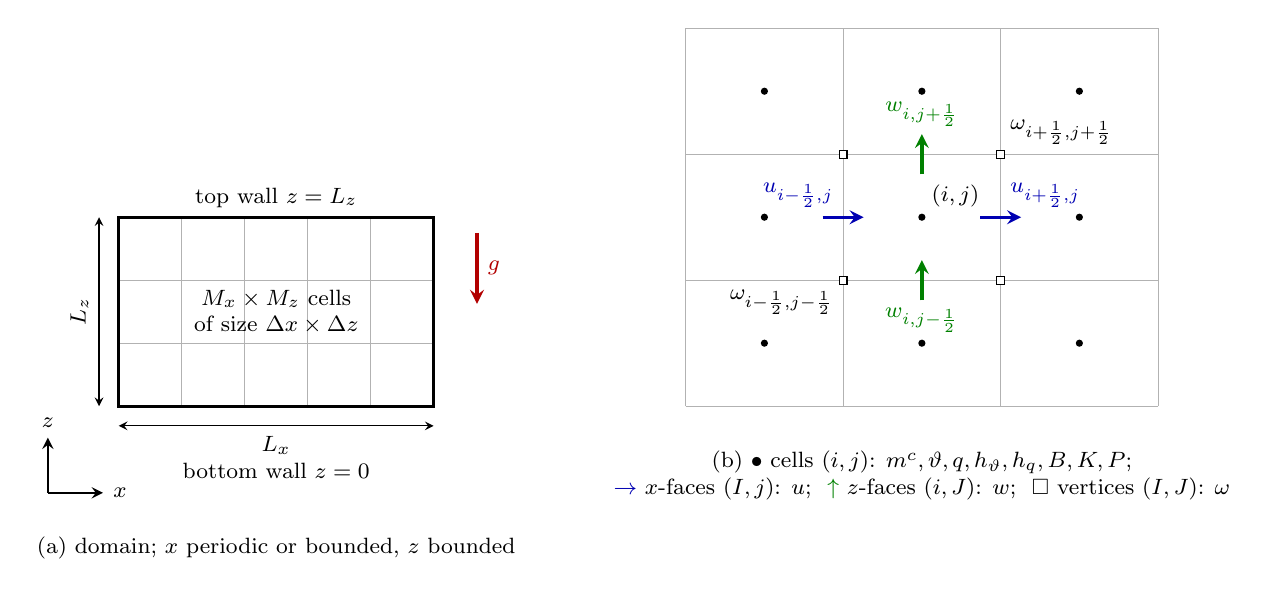
\begin{tikzpicture}[>=stealth,font=\footnotesize]
% (a) domain geometry
\begin{scope}
  \draw[gray!60] (0,0) grid[step=0.8] (4,2.4);
  \draw[very thick] (0,0) rectangle (4,2.4);
  \node at (2,-0.5) {$L_x$};
  \node[rotate=90] at (-0.5,1.2) {$L_z$};
  \draw[<->] (0,-0.25) -- (4,-0.25);
  \draw[<->] (-0.25,0) -- (-0.25,2.4);
  \draw[->,thick] (-0.9,-1.1) -- (-0.2,-1.1) node[right] {$x$};
  \draw[->,thick] (-0.9,-1.1) -- (-0.9,-0.4) node[above] {$z$};
  \draw[->,very thick,red!70!black] (4.55,2.2) -- (4.55,1.3) node[midway,right] {$g$};
  \node[above] at (2,2.4) {top wall $z=L_z$};
  \node[align=center] at (2,1.2) {$M_x\times M_z$ cells\\of size $\Delta x\times\Delta z$};
  \node[below] at (2,-0.6) {bottom wall $z=0$};
  \node[align=center] at (2,-1.8) {(a) domain; $x$ periodic or bounded, $z$ bounded};
\end{scope}
% (b) C-grid stencil
\begin{scope}[xshift=7.2cm,x=2.0cm,y=1.6cm,font=\footnotesize]
  \draw[gray!60] (0,0) grid[step=1] (3,3);
  \foreach \a in {0.5,1.5,2.5} \foreach \b in {0.5,1.5,2.5} \fill (\a,\b) circle (1.3pt);
  \node[above right] at (1.5,1.5) {$(i,j)$};
  % u on x-faces
  \foreach \xx in {1,2} \draw[->,very thick,blue!70!black] (\xx-0.13,1.5)--(\xx+0.13,1.5);
  \node[blue!70!black,above left] at (1,1.5) {$u_{i-\frac12,j}$};
  \node[blue!70!black,above right] at (2,1.5) {$u_{i+\frac12,j}$};
  % w on z-faces
  \foreach \yy in {1,2} \draw[->,very thick,green!50!black] (1.5,\yy-0.16)--(1.5,\yy+0.16);
  \node[green!50!black,above] at (1.5,2.14) {$w_{i,j+\frac12}$};
  \node[green!50!black,below] at (1.5,0.86) {$w_{i,j-\frac12}$};
  % vertices
  \foreach \xx in {1,2} \foreach \yy in {1,2} \node[draw,fill=white,inner sep=1.4pt] at (\xx,\yy) {};
  \node[above right] at (2,2) {$\omega_{i+\frac12,j+\frac12}$};
  \node[below left] at (1,1) {$\omega_{i-\frac12,j-\frac12}$};
  \node[align=center,font=\footnotesize] at (1.5,-0.55) {(b) $\bullet$ cells $(i,j)$: $m^c,\vartheta,q,h_\vartheta,h_q,B,K,P$;\\
        {\color{blue!70!black}$\rightarrow$} $x$-faces $(I,j)$: $u$;\ \ {\color{green!50!black}$\uparrow$} $z$-faces $(i,J)$: $w$;\ \ $\square$ vertices $(I,J)$: $\omega$};
\end{scope}
\end{tikzpicture}
\caption{(a) The box and its cell grid, with gravity along $-z$. (b) The C-grid around cell $(i,j)$: scalars at cell centres, $u$ on $x$-faces, $w$ on $z$-faces, vorticity at vertices. Cell indices $i,j$ are integers; face and vertex (dual) indices $I,J$ are half-integers.}
\label{fig:grid}
\end{figure}

\subsection{Primal and dual indices}\label{sec:indices}
\textbf{Primal} indices $i,j$ are integers and number the cells; \textbf{dual} indices $I,J$ are half-integers and number the faces. The two $x$-faces of cell $i$ are the \emph{left} face $I=i-\tfrac12$ and the \emph{right} face $I=i+\tfrac12$; the two $z$-faces of cell $j$ are the \emph{bottom} face $J=j-\tfrac12$ and the \emph{top} face $J=j+\tfrac12$.
Conversely, face $I$ lies between cells $i=I-\tfrac12$ (on its left) and $i=I+\tfrac12$ (on its right), and face $J$ between cells $j=J-\tfrac12$ (below) and $j=J+\tfrac12$ (above). A vertex is $(I,J)$, the corner shared by the cells $(I\pm\tfrac12,J\pm\tfrac12)$. For any index $k$ (primal or dual) along $x$ or $z$ the coordinate is
\begin{equation}
  x_k=(k-\tfrac12)\Delta x,\qquad z_k=(k-\tfrac12)\Delta z ,
\end{equation}
so that cell $i$ is centred at $x_i=(i-\tfrac12)\Delta x$ and the face $I=i-\tfrac12$ at $x_I=(i-1)\Delta x$.
Interior cells are $i=1,\dots,M_x$, $j=1,\dots,M_z$. A bounded direction has $M+1$ faces, $I=\tfrac12,\tfrac32,\dots,M_x+\tfrac12$, the first and last being the walls (at $x=0$ and $x=L_x$); a periodic direction has $M$ faces,
$I=\tfrac12,\dots,M_x-\tfrac12$, with $M_x+\tfrac12\equiv\tfrac12$. The $z$ direction is always bounded.
Indices outside the interior are \emph{ghost} (halo) indices; the halo width $H\ge1$ only needs to contain the stencils.
In the code, the array index is $i+H$ for a cell index and $I+\tfrac12+H$ for a face index (the code's face index $n$ is the face on the left of cell $n$).

The location of each field follows from whether each index is primal or dual:
\begin{center}\small
\begin{tabular}{lll}
\hline
Location & Indices & Fields \\ \hline
cell centre & $(i,j)$ & $m^c$, $\vt,q,T,\hth,\hq,c_p,\Gamma,B,P$, $K$, $D$, $\rho\varepsilon$, $\sigma_\vt$, $p$, $\tau_{xx},\tau_{zz}$ \\
$x$-face & $(I,j)$ & $u$, $F_x$, $\mathcal G_x$, $J_{\vt;x}$, $J_{q;x}$, $(\bu\!\cdot\!\btau)_x$, $S_x$, $\rho^u$ \\
$z$-face & $(i,J)$ & $w$, $F_z$, $\mathcal G_z$, $J_{\vt;z}$, $J_{q;z}$, $(\bu\!\cdot\!\btau)_z$, $S_z$, $\rho^w$ \\
vertex & $(I,J)$ & $\omega$, $\tau_{xz}$, $\zeta$ \\ \hline
\end{tabular}
\end{center}
The tracer array is $m^c_{i,j}$: $(m^\vt,m^q)=(\rho_R\vt,\rho_Rq)$ in AN2D, and $(m^\rho,m^\vt,m^q)=(\rho,\rho\vt,\rho q)$ in FC2D (code \code{m[i,j,c]}).

\subsection{Difference and average operators}\label{sec:ops}
For an array $a$ with an index $k$ along $x$ (integer or half-integer), define
\begin{equation}
  (\dx a)_{k}=a_{k+\frac12}-a_{k-\frac12},\qquad (\Ix a)_{k}=\tfrac12\big(a_{k+\frac12}+a_{k-\frac12}\big),
\end{equation}
and identically $\dz,\Iz$ along $z$. The result lives at index $k$ whose type (primal/dual) is the opposite of that of $a$: $\dx$ and $\Ix$ map $x$-faces to cells and cells to $x$-faces, e.g.\ $(\dx u)_{i,j}=u_{i+\frac12,j}-u_{i-\frac12,j}$ and
$(\dx q)_{I,j}=q_{I+\frac12,j}-q_{I-\frac12,j}$. Averages across both directions compose, $\Ixz=\Ix\Iz$ (cells to vertices, or $x$-faces to $z$-faces). The \emph{discrete derivatives}
\begin{equation}
  \partial_x=\Delta x^{-1}\dx,\qquad \partial_z=\Delta z^{-1}\dz
\end{equation}
are used from now on, as are $\Ix,\Iz$; formulas are written with these operators instead of explicit differences. A vertical profile $f_j$ (such as $\rho_R$) is a field independent of $i$: $(\Iz f)_J=\tfrac12(f_{J-\frac12}+f_{J+\frac12})$.
All operators are the second-order centred scheme (\code{Centred2}). The identities they satisfy are stated in \S\ref{sec:econs}.

\subsection{Halos and the state boundary conditions}\label{sec:halo}
Before every tendency evaluation the halo of the state is rebuilt from its interior (\code{state\_bc!}); the interior is never changed except that wall-face normal velocities are set to $0$.
Directions are treated in the order $x$ then $z$, each over the full extent (ghosts included) of the other direction, so corner ghosts are filled in the second pass.
\paragraph{Periodic direction.} Indices are taken modulo $M$: $a_{k}\equiv a_{k+M}$.
\paragraph{Bounded direction, primal-type index} (cell fields; the tangential velocity component): for $h=1,\dots,H$,
$a_{1-h}=\mathrm{g}_{\rm lo}(a_h,d)$ and $a_{M+h}=\mathrm{g}_{\rm hi}(a_{M+1-h},d)$, with $d=(2h-1)\Delta$ the distance between the ghost and its mirror image.
\paragraph{Bounded direction, dual-type index} (the wall-normal velocity): $a_{\frac12}=a_{M+\frac12}=0$ and, for $h=1,\dots,H$, $a_{\frac12-h}=-a_{\frac12+h}$ and $a_{M+\frac12+h}=-a_{M+\frac12-h}$ (odd about the wall).
\paragraph{Ghost rules $\mathrm g$.} For tracers $m^c$ (and all derived thermodynamic fields) the rule is \emph{zero gradient}, $\mathrm g(v,d)=v$. For the tangential velocity at a wall:
\begin{center}\small
\begin{tabular}{ll}
\hline
free slip & $v_{\rm g}=v$\\
no slip & $v_{\rm g}=-v$\\
moving wall, speed $U_t$ & $v_{\rm g}=2U_t-v$\\
prescribed stress $\tau_w$ & $v_{\rm g}=v+d\,\tau_w/\eta$\\ \hline
\end{tabular}
\end{center}
where $\tau_w=\eta\,\partial v/\partial n_{\rm out}$ with $n_{\rm out}$ the outward normal coordinate, so that the centred difference across the wall realises the condition. $U_t$ is positive along $+x$ on bottom/top walls and along $+z$ on left/right walls.
\paragraph{Sampling of wall data.} Wall data given as functions of the position along the wall are evaluated once, at the position of the field they apply to: tracer data (flux, heat flux, value) at the cell-centre coordinate $x_i$ or $z_j$ along the wall, and the tangential velocity or stress at the coordinate of that velocity component along the wall ($z_J$ for $w$ on a left/right wall, $x_I$ for $u$ on a bottom/top wall).
Numbers are used as they are.

\subsection{Evaluation ranges}\label{sec:ranges}
In the kernels below, (i) cell fields are evaluated at interior cells; (ii) $x$-face fields at all interior $x$-faces $I$ (including wall faces) and $j=1,\dots,M_z$; (iii) $z$-face fields at $i=1,\dots,M_x$ and all interior $z$-faces $J$; (iv) vertex fields at all interior $I,J$ (including wall vertices).
Derived fields (all but the state) needed at ghost cells receive the zero-gradient rule (or periodic wrap); they are
read only to produce zero (differences across a wall) or in wall-face quantities that are overwritten or multiplied by the zero wall-normal velocity. Ghost values of the \emph{state} do matter: they determine the vertices on the walls ($\omega$, $\tau_{xz}$, $\zeta$).

\section{The tendency computation}\label{sec:shared}
\code{tendencies!(dstate, scratch, model, state, t)} returns the time derivative of $(m,u,w)$ as follows. Let $\rho^c,\rho^u,\rho^w$ be the cell and face densities that weight the mass fluxes and the kinetic energy, and $v^u=1/\rho^u$, $v^w=1/\rho^w$:
\begin{center}\small
\begin{tabular}{lccc}
\hline
 & $\rho^c_{i,j}$ & $\rho^u_{I,j}$ & $\rho^w_{i,J}$ \\ \hline
AN2D & $\rho_{R,j}$ & $\rho_{R,j}$ & $(\Iz\rho_R)_J$ \\
FC2D & $m^\rho_{i,j}$ & $(\Ix m^\rho)_{I,j}$ & $(\Iz m^\rho)_{i,J}$ \\ \hline
\end{tabular}
\end{center}
In every case $\rho^u=\Ix\rho^c$ and $\rho^w=\Iz\rho^c$. (AN2D uses the reference density in the halo cells $j=0$, $j=M_z+1$, \S\ref{sec:ref}; FC2D uses the zero-gradient ghost density.)

\subsection{Step 0: halo of the state}
As in \S\ref{sec:halo}.

\subsection{Step 1: thermodynamics}
At interior cells, then zero-gradient/periodic halo of every result. For each $(i,j)$:
\begin{itemize}
  \item AN2D: $\vt=m^\vt/\rho_{R,j}$, $q=m^q/\rho_{R,j}$, $P=P_{R,j}$.
  \item FC2D: $\rho=m^\rho$, $\vt=m^\vt/\rho$, $q=m^q/\rho$, $P=P(1/\rho,\vt,q)$ from the fluid.
\end{itemize}
Then $T,\hth,\hq,c_p,\partial_q\vt|_{P,T}$ are the fluid functions of $(P,\vt,q)$, $B=h(P,\vt,q)-\vt\hth-q\hq$ and, with $(\partial_P\mu,\partial_q\mu)$ the fluid functions of $(P,T,q)$,
\begin{equation}
  \Gamma=-\frac{\partial_P\mu}{\partial_q\mu}\qquad\text{(both models).}
\end{equation}
With the buoyancy options of AN2D, $B$ is replaced by the buoyancy $b$: $b=g(\rho_Rv-1)$ (consistent) or $g(1-1/(\rho_Rv))$ (traditional), with $v=v(P_{R,j},\vt,q)$.

\subsection{Step 2: kinematics}
\begin{equation}
  D=\partial_xu+\partial_zw\ \ (\text{cells}),\qquad
  \omega=\partial_zu-\partial_xw\ \ (\text{vertices}),\qquad
  K=\tfrac12\big(\Ix(u^2)+\Iz(w^2)\big)\ \ (\text{cells}),
\end{equation}
where $K$ is the average of the squares, not the square of the averages.

\subsection{Step 3: advective fluxes}
Centred, flux form, for each tracer $c$ of $m$ (and the mass flux $\mathcal M$):
\begin{equation}
  \mathcal G^c_x=u\,\Ix m^c,\qquad \mathcal G^c_z=w\,\Iz m^c,\qquad
  \mathcal M_x=\rho^uu,\quad\mathcal M_z=\rho^ww .
\end{equation}
In FC2D $\mathcal M=\mathcal G^\rho$ (since $\rho^u=\Ix m^\rho$); in AN2D $\mathcal M_x=\rho_Ru$ is not stored.

\subsection{Step 4: vortex force}
The force $\bomega\times\bu=(S_x,S_z)=(\omega w,-\omega u)$ is discretised in the energy-conserving form of Sadourny (1975):
\begin{equation}
  \zeta=\frac{\omega}{\Ixz\rho^c},\qquad U^v=\Iz\mathcal M_x,\quad W^v=\Ix\mathcal M_z\quad(\text{at vertices}),\qquad
  S_x=\Iz(\zeta\,W^v),\quad S_z=-\Ix(\zeta\,U^v).
\end{equation}
(For AN2D, $\Ixz\rho^c=\Iz\rho_R$.) Products are formed at vertices and then averaged to the faces. Sadourny's other scheme and Arakawa--Lamb's are also implemented in \code{CFBoxes} but are not specified here.

\subsection{Step 5: viscous stress}
\begin{equation}
  \tau_{xx}=2\eta\big(\partial_xu-\tfrac13D\big),\quad\tau_{zz}=2\eta\big(\partial_zw-\tfrac13D\big)\ \ (\text{cells}),\qquad
  \tau_{xz}=\eta\big(\partial_zu+\partial_xw\big)\ \ (\text{vertices}).
\end{equation}
The energy flux $\bu\cdot\btau$ and the force $\bF$ (in the rotational form of \eqref{eq:tau}) at the faces are
\begin{align}
  (\bu\!\cdot\!\btau)_x&=u\,\Ix\tau_{xx}+\Iz\big((\Ix w)\,\tau_{xz}\big), &
  (\bu\!\cdot\!\btau)_z&=w\,\Iz\tau_{zz}+\Ix\big((\Iz u)\,\tau_{xz}\big),\\
  F_x&=\eta\big(\partial_z\omega+\tfrac43\partial_xD\big), &
  F_z&=\eta\big(-\partial_x\omega+\tfrac43\partial_zD\big).
\end{align}
At wall vertices $\Ix w$ and $\Iz u$ contain the ghost values, so the wall stress work is that of the tangential wall velocity.
The dissipation at interior cells is
\begin{equation}
  \rho\varepsilon=\partial_x(\bu\!\cdot\!\btau)_x+\partial_z(\bu\!\cdot\!\btau)_z-\Ix(uF_x)-\Iz(wF_z).
  \label{eq:rhoeps}
\end{equation}

\subsection{Step 6: diffusive fluxes}
The density in the fluxes is the face density of the table above, $\rho^u$ at $x$-faces and $\rho^w$ at $z$-faces. Coefficients at faces are $\Ix$ or $\Iz$ of the cell values. The pressure gradient in the barodiffusion term is that of $P_f$, the pressure of the model: $P_f=P$ in FC2D (a cell field) and $P_f=P_R$ in AN2D, a profile with
\begin{equation}
  \partial_xP_R=0,\qquad \partial_zP_R=-g\,\Iz\rho_R=-g\rho^w\quad\text{exactly (\S\ref{sec:ref})}.
\end{equation}
Then, at $x$-faces,
\begin{align}
  J_{q;x}&=-\rho^u\kappa_q\big(\partial_xq-(\Ix\Gamma)\,\partial_xP_f\big),\\
  J_{\vt;x}&=-\frac{\rho^u\,\kappa_T\,(\Ix c_p)\,\partial_xT}{\Ix\hth}+(\Ix\partial_q\vt)\,J_{q;x},
\end{align}
and the same at $z$-faces with $\rho^w$, $\Iz$, $\partial_z$ (with $\partial_zP_f$). The diffusive heating at faces is
\begin{equation}
  H_x=-\big(J_{\vt;x}\,\partial_x\hth+J_{q;x}\,\partial_x\hq\big),\qquad H_z=-\big(J_{\vt;z}\,\partial_z\hth+J_{q;z}\,\partial_z\hq\big).
\end{equation}
At wall faces the fluxes are overwritten by the boundary conditions (\S\ref{sec:wallflux}); at a wall face the ghost values of $\hth,\hq$ equal the cell values, so $H=0$ there. The production of $\rho\vt$ at interior cells (consistent fluxes) is
\begin{equation}
  \sigma_\vt=\frac{\rho\varepsilon+\Ix H_x+\Iz H_z}{\hth},
  \label{eq:sigmad}
\end{equation}
the discrete form of \eqref{eq:sigma}. With the down-gradient option: $J_{q;x}=-\rho^u\kappa_q\partial_xq$, $J_{\vt;x}=-\rho^u\kappa_T\partial_x\vt$ (and in $z$), $\sigma_\vt=0$.

\subsection{Step 7: momentum tendencies}
Before the pressure correction, at interior $x$-faces $(I,j)$ and $z$-faces $(i,J)$ (the wall faces are set in step 10):
\begin{align}
  \dot u&=-v^u\Big[(\Ix m^\vt)\,\partial_x\hth+(\Ix m^q)\,\partial_x\hq\Big]-\partial_x\big(B+K\big)-S_x+v^uF_x,
  \label{eq:udot}\\
  \dot w&=-v^w\Big[(\Iz m^\vt)\,\partial_z\hth+(\Iz m^q)\,\partial_z\hq\Big]-\partial_z\big(B+K+\Phi\big)-S_z+v^wF_z,
  \label{eq:wdot}
\end{align}
with $\Phi_j=g(z_j-z_0)$, for which $\partial_z\Phi=g$ exactly. Here $B=h-\vt\hth-q\hq$ is the Bernoulli potential of step 1; $m^\vt,m^q$ are the tracer densities ($m^1,m^2$ in AN2D, $m^2,m^3$ in FC2D), so that $v^u\Ix m^\vt$ is the discrete $\vt$ at the $x$-face.
In AN2D, with a buoyancy option ($B\to b$ computed in step 1), instead
\begin{equation}
  \dot u=-\partial_xK-S_x+v^uF_x,\qquad\dot w=\Iz b-\partial_zK-S_z+v^wF_z .
\end{equation}
The arrays are wrapped in periodic directions.

\subsection{Step 8 (AN2D only): pressure correction}
The reduced pressure $p$, and $\dot u\leftarrow\dot u-\partial_xp$, $\dot w\leftarrow\dot w-\partial_zp$ at all faces; see \S\ref{sec:poisson}.

\subsection{Step 9: tracer tendencies}
At interior cells,
\begin{equation}
  \dot m^c=-\partial_x\big(\mathcal G^c_x+J^c_x\big)-\partial_z\big(\mathcal G^c_z+J^c_z\big)+\sigma^c,
  \label{eq:mdot}
\end{equation}
with $J^\rho=0$, $\sigma^\rho=\sigma^q=0$, $J^\vt=J_\vt$, $J^q=J_q$, $\sigma^\vt=\sigma_\vt$ (the mass $m^\rho$ exists only in FC2D).

\subsection{Step 10: tendency boundary conditions}
Set to zero: $\dot m$ in the halo, $\dot u,\dot w$ in the halo, $\dot u$ on $x$-walls and $\dot w$ on $z$-walls. The state is not otherwise modified.

\section{Wall conditions on the fluxes}\label{sec:wallflux}
After step 6, on each wall face the fluxes $J_\vt,J_q$ are replaced, at every position along the wall, by the following. Let $n=+1$ (lower wall: $I=\tfrac12$ or $J=\tfrac12$) or $n=-1$ (upper: $I=M_x+\tfrac12$ or $J=M_z+\tfrac12$) be the inward normal, $i_c$ the adjacent cell ($i=1$ or $M_x$, $j=1$ or $M_z$), $d=\Delta/2$ the half-cell distance; fluxes are in the coordinate direction. The wall state $(\rho_w,P_w,\partial P_{f;w})$ (wall density, wall pressure and the wall value of the gradient $\partial P_f$ used in the composition flux) is:
\begin{center}\small
\begin{tabular}{lll}
\hline
 & AN2D & FC2D \\ \hline
$x$-wall & $\rho_{R,j},\ P_{R,j},\ 0$ & $\rho_{i_c},\ P_{i_c},\ 0$ \\
$z$-wall & $(\Iz\rho_R)_J,\ P_{R,j}+n\rho_{R,j}g\,d,\ -(\Iz\rho_R)_Jg$ & $\rho_{i_c},\ P_{i_c}+n\rho_{i_c}g\,d,\ -\rho_{i_c}g$ \\ \hline
\end{tabular}
\end{center}
\begin{itemize}
  \item \textbf{Composition.} Prescribed flux $F$ of $\rho q$: $J_q=nF$. Prescribed wall value $q_w$: $J_q=-\rho_w\kappa_q\big(n(q_{i_c}-q_w)/d-\Gamma_{i_c}\,\partial P_{f;w}\big)$.
  \item $\vt$. Prescribed flux $F$ of $\rho\vt$: $J_\vt=nF$. Prescribed heat flux $F$ (reduced heat flux into the fluid): $J_\vt=nF/\hth_{i_c}+\partial_q\vt_{i_c}\,J_q$. Prescribed value $\vt_w$:
  $J_\vt=-\rho_w\,c_{p;i_c}\kappa_T\,n(T_{i_c}-T_w)/(d\,\hth_{i_c})+\partial_q\vt_{i_c}J_q$ with $T_w=T(P_w,\vt_w,q_{i_c})$.
\end{itemize}
Because the ghost values of $\hth$ and $\hq$ equal the cell values, the energy delivered by a wall is $\hth_{i_c}J_\vt+\hq_{i_c}J_q$ (with the sign convention of \eqref{eq:wallinput}), which for a heat-flux wall is $F+\partial_qh|_{P,T}J_qn$.

\section{Pressure projection and the Poisson solver (AN2D)}\label{sec:poisson}
\subsection{The discrete problem}
After step 7 let $(\dot u,\dot w)$ be the tendencies. First set $\dot u=0$ on $x$-walls and $\dot w=0$ on $z$-walls. Define the weighted divergence and the operator $L$ on interior cells:
\begin{align}
  r&=\rho_R\,\partial_x\dot u+\partial_z\big(\rho^w\dot w\big),\\
  Lp&=\rho_R\,\partial_x\partial_xp+\partial_z\big(\rho^w\,\partial_zp\big),
  \label{eq:Lp}
\end{align}
and find $p$ at interior cells with $Lp=r$. In \eqref{eq:Lp} the ghost values of $p$ are the zero-gradient ones, $p_{0,j}=p_{1,j}$, $p_{M_x+1,j}=p_{M_x,j}$ for bounded $x$ (periodic wrap otherwise) and $p_{i,0}=p_{i,1}$, $p_{i,M_z+1}=p_{i,M_z}$ in $z$, which makes the gradient of $p$ vanish on the walls.
Written out, $(Lp)_{i,j}=\rho_{R,j}(p_{i+1,j}-2p_{i,j}+p_{i-1,j})/\Delta x^2+\big[\rho^w_{j+\frac12}(p_{i,j+1}-p_{i,j})-\rho^w_{j-\frac12}(p_{i,j}-p_{i,j-1})\big]/\Delta z^2$.

\paragraph{Projection.} Let $G p=(\partial_xp,\partial_zp)$ at faces (zero on wall faces). Then, directly from the definitions, $L=\mathrm{div}_\rho\circ G$ where $\mathrm{div}_\rho(a,b)=\rho_R\partial_xa+\partial_z(\rho^wb)$. Hence
$\mathrm{div}_\rho\big((\dot u,\dot w)-Gp\big)=r-Lp=0$, and the corrected tendency has zero wall-normal component. In the code the gradients at wall faces are $0$ because the ghost value of $p$ equals the cell value, and the correction is applied at all faces.

\paragraph{Properties of $L$.} (i) $L$ is symmetric for the unweighted inner product $\langle a,b\rangle=\sum_{i,j}a_{i,j}b_{i,j}$: the $x$-part is $\rho_{R,j}$ times the same symmetric second difference in each row, the $z$-part is a symmetric conductance matrix with weights $\rho^w$.
(ii) $L$ is negative semi-definite: by summation by parts (\S\ref{sec:econs}), $\langle p,Lp\rangle=-\sum_{I,j}\rho_{R,j}(\partial_xp)^2-\sum_{i,J}\rho^w_J(\partial_zp)^2\le0$, sums over interior faces. (iii) The kernel is the constants: $\langle p,Lp\rangle=0$ forces all differences to vanish. (iv) $\sum_{i,j}(Lp)_{i,j}=0$ for all $p$, hence
$Lp=r$ is solvable iff $\sum_{i,j}r_{i,j}=0$. This holds: $\sum_ir_{i,j}$ telescopes in $x$ (periodic wrap or zero wall velocity), and $\sum_j$ telescopes in $z$ since $\dot w=0$ at both walls.
The solution is unique up to a constant, fixed by the gauge below.

\subsection{Diagonalisation in $x$}
Write $L=\rho_R\otimes A_x+\mathrm{Id}\otimes T_z$ where $A_x$ is the $x$-second difference (acting within a row) and $T_z$ the tridiagonal $z$-operator (acting within a column). Since $T_z$ does not depend on $i$ and $\rho_{R,j}$ does not depend on $i$,
any orthogonal basis diagonalising $A_x$ with eigenvalues $\lambda_m$ decouples $L$ into independent tridiagonal systems in $j$, one per mode $m$.
\begin{itemize}
  \item \emph{Periodic} $x$: eigenvectors $e^{2\pi\mathrm i\,m(i-1)/M_x}$, $m=0,\dots,M_x-1$; $(e^{\mathrm i\theta(i+1)}-2e^{\mathrm i\theta i}+e^{\mathrm i\theta(i-1)})/\Delta x^2=-\frac{4\sin^2(\theta/2)}{\Delta x^2}e^{\mathrm i\theta i}$ with $\theta=2\pi m/M_x$,
        so $\lambda_m=-\big(2\sin(\pi m/M_x)/\Delta x\big)^2$, which is also the value for $M_x-m$ (conjugate modes).
  \item \emph{Bounded} $x$ (Neumann ghosts $p_0=p_1$, $p_{M+1}=p_M$): eigenvectors $\cos\!\big(\pi m(i-\tfrac12)/M_x\big)$, $m=0,\dots,M_x-1$ (discrete cosine transform of type II). Check: both ghost conditions hold for these (e.g.\ $p_0=\cos(\pi m/2M_x)=p_1$), and the three-term sum equals
        $2\cos(\cdot)\big(\cos(\pi m/M_x)-1\big)$, so $\lambda_m=-\big(2\sin(\pi m/(2M_x))/\Delta x\big)^2$.
\end{itemize}
In both cases $\lambda_0=0$ and $\lambda_m<0$ otherwise.

\paragraph{Transforms as implemented (FFTW conventions).}
\begin{itemize}
  \item Periodic $x$: forward = real-to-complex FFT (\code{rfft}) giving $\lfloor M_x/2\rfloor+1$ complex coefficients $\hat r_m=\sum_{i=1}^{M_x}r_i\,e^{-2\pi\mathrm i\,m(i-1)/M_x}$; backward = complex-to-real (\code{brfft}, unnormalised), which reconstructs the real signal from the half spectrum assuming Hermitian symmetry,
        so that backward$\circ$forward $=M_x\cdot\mathrm{id}$. The real and imaginary parts of the half spectrum are stored interleaved, giving $2(\lfloor M_x/2\rfloor+1)$ \emph{real rows}, each a real tridiagonal system with the same $\lambda_m$. The imaginary parts of $m=0$ (and of $m=M_x/2$ for even $M_x$) do not enter the backward transform.
  \item Bounded $x$: forward = DCT-II (\code{REDFT10}): $\hat r_m=2\sum_{i=1}^{M_x}r_i\cos(\pi m(i-\tfrac12)/M_x)$; backward = DCT-III (\code{REDFT01}), with backward$\circ$forward $=2M_x\cdot\mathrm{id}$.
\end{itemize}
Let $s$ be $M_x$ (periodic) or $2M_x$ (bounded). The code multiplies the right-hand side by $1/s$ when forming $r$, so that after the backward transform the result is $p$ itself.

\subsection{Tridiagonal solve in $z$ (Thomas algorithm)}
For each real row (mode $m$) the system at levels $j=1,\dots,M_z$ is
\begin{equation}
  a_j\hat p_{j-1}+b_j\hat p_j+c_j\hat p_{j+1}=\hat r_j,\qquad
  a_j=\frac{\rho^w_{j-\frac12}}{\Delta z^2},\quad c_j=\frac{\rho^w_{j+\frac12}}{\Delta z^2},\quad b_j=\lambda_m\rho_{R,j}-a_j-c_j,
\end{equation}
with $a_1=0$ and $c_{M_z}=0$ (no flux through the walls). The factorisation is precomputed once per model (it depends only on $\rho_R$ and $\Delta$): pivots $\mathrm{pv}_1=b_1$, $\mathrm{pv}_j=b_j-a_j\,f_{j-1}$ with $f_j=c_j/\mathrm{pv}_j$, and $\mathrm{ip}_j=1/\mathrm{pv}_j$. The solve is:
\begin{align}
  y_1&=\hat r_1\,\mathrm{ip}_1, & y_j&=(\hat r_j-a_jy_{j-1})\,\mathrm{ip}_j\quad(j=2,\dots,M_z),\\
  \hat p_{M_z}&=y_{M_z}, & \hat p_j&=y_j-f_j\hat p_{j+1}\quad(j=M_z-1,\dots,1).
\end{align}

\subsection{Gauge}
For $\lambda_m=0$ ($m=0$; both its real rows) the matrix is singular: $b_j=-a_j-c_j$, and the rows sum to zero because $c_j=a_{j+1}$ and $a_1=c_{M_z}=0$.
The factorisation is computed level by level as above, but for these rows the level-one values are overwritten right after level one is processed, $f_1\leftarrow0$ and $\mathrm{ip}_1\leftarrow0$, so that $\mathrm{pv}_2=b_2$. The solve then gives $y_1=0$, $y_2=\hat r_2/b_2$, \dots, and back substitution gives
$\hat p_1=y_1-f_1\hat p_2=0$. In effect the level-one equation is discarded and $\hat p_1=0$ is imposed, so \emph{the horizontal mean of $p$ on the bottom level is zero}. Because the rows sum to zero, the discarded equation is the negative of the sum of the retained ones,
and is therefore satisfied exactly when $\sum_j\hat r_j=0$ for the mean mode, which is property (iv). The total pressure is $P=P_R+\rho_Rp$, defined up to this gauge. The user may add a constant to $p$ after the solve (\code{gauge\_offset}, default $0$, so that the horizontal mean of $p$ on the bottom level is the offset). It changes the pressure but no tendency, and no term of the energy budget except the fluxes $\rho_R\Sigma\mathbf u$ and $(P-P_R)\mathbf u$, which change by the constant times the mass flux; their divergences do not, since $\nabla\!\cdot(\rho_R\mathbf u)=0$ discretely (tested).

\subsection{Assembly}
The steps in \code{pressure!}: (1) zero the wall-normal $\dot u,\dot w$ on the walls; (2) form $r/s$ at interior cells; (3) forward transform each level $j$ in $x$; (4) Thomas solve each row; (5) backward transform;
(6) copy into the interior of $p$ and set the halo of $p$ by zero gradient/periodic wrap; (7) $\dot u\leftarrow\dot u-\partial_xp$ at all $x$-faces, $\dot w\leftarrow\dot w-\partial_zp$ at all $z$-faces.
In step 7 the wall faces receive $0$ from the zero-gradient halo, so the corrected tendency has zero wall-normal component.

\section{Anelastic reference state and initialisation (AN2D)}\label{sec:ref}
\subsection{Reference state}
The reference state is held at the cell centres of the \emph{full} vertical axis, halo included, $j=1-H,\dots,M_z+H$:
\begin{itemize}
  \item $\rho_{R,j}$: a number $\rho_0$; or a function $\rho_R(z)$ evaluated at the cell centres $z_j$ (also in the halo, i.e.\ the function is extrapolated); or a vector of $M_z$ values, extended into the halo by repeating its end values.
  \item $P_{R,j}$: hydrostatic, $P_{R,j}-P_{R,j-1}=-g\Delta z\,\Iz\rho_R$ between the centres $j-1$ and $j$ (the density of the face between them is the average of the two cells), up to a constant fixed by the anchor. The pressure at $z_0$ is that of the piecewise-linear interpolant of the cell-centre values $P_{R,j}$, taken in the segment between two interior cells that contains $z_0$ (linearly extrapolated from the nearest segment if $z_0$ is outside the box), and it equals $P_{\rm ref}$.
\end{itemize}
Consequently $\partial_zP_R=-g\,\Iz\rho_R=-g\rho^w$ exactly: the discrete hydrostatic balance uses the face density $\rho^w$ that weights the vertical mass flux and the Poisson operator. FC2D has no reference state; its balanced rest density (\code{balanced\_density}) has the pressure $P_{\rm ref}$ at $z_0$ in the same sense, the pressure at the top cell being found by secant iterations on the interpolated pressure at $z_0$.
The specific volume is not stored; face values of $\rho_R$ are $\Iz\rho_R$.

\subsection{Initial state}
Given $\vt(x,z)$ and $q(x,z)$: $m^\vt_{i,j}=\rho_{R,j}\vt(x_i,z_j)$, $m^q_{i,j}=\rho_{R,j}q(x_i,z_j)$ at every cell including the halo (then replaced by the halo rule, \S\ref{sec:halo}). The velocity is either zero or given by face arrays. A discretely divergence-free velocity is obtained from a mass streamfunction $\psi(x,z)$ [kg\,m$^{-1}$s$^{-1}$] evaluated at the vertices $(x_I,z_J)$:
\begin{equation}
  \rho^uu=\partial_z\psi,\qquad \rho^ww=-\partial_x\psi,
\end{equation}
so that $\mathrm{div}(\rho^uu,\rho^ww)=\partial_x\partial_z\psi-\partial_z\partial_x\psi=0$ identically. The wall-normal velocity vanishes if $\psi$ is constant along the wall.
Energy conservation of AN2D requires a state on this constraint manifold (\S\ref{sec:econs}).

\section{Time integration}
Both models are advanced with the classical fourth-order Runge--Kutta scheme in the following (low-storage) form, with $f$ the tendency map and $\Delta t$ the step; all state arrays are updated at every point including the halo, which is then rebuilt at each evaluation of $f$:
\begin{align}
  k_0&=f(\mathbf s^n), & \mathbf s_1&=\mathbf s^n+\tfrac{\Delta t}2k_0, & k_1&=f(\mathbf s_1),\\
  \mathbf s_2&=\mathbf s_1-\tfrac{\Delta t}2k_0+\tfrac{\Delta t}2k_1, & k_2&=f(\mathbf s_2), & &\\
  \mathbf s_3&=\mathbf s_2-\tfrac{\Delta t}2k_1+\Delta t\,k_2, & k_3&=f(\mathbf s_3), & &\\
  \mathbf s^{n+1}&=\mathbf s_3+\tfrac{\Delta t}6k_0+\tfrac{\Delta t}3k_1-\tfrac{2\Delta t}3k_2+\tfrac{\Delta t}6k_3, & & & &
\end{align}
i.e.\ $\mathbf s_2=\mathbf s^n+\frac{\Delta t}2k_1$, $\mathbf s_3=\mathbf s^n+\Delta t\,k_2$ and $\mathbf s^{n+1}=\mathbf s^n+\frac{\Delta t}6(k_0+2k_1+2k_2+k_3)$. A five-stage Kinnmark--Gray scheme is also available and is not specified here.
Time is advanced in slices of fixed length $\tau_s$ (the output interval). At the start of each slice
\begin{equation}
  \Delta t=\frac{\tau_s}{\lceil\tau_s/\min(C\,\sqrt8/\omega_{\max},\,\tau_s,\,\Delta t_{\max})\rceil},
\end{equation}
where $C\le1$ is the Courant number, $\sqrt8$ the stability limit of RK4 on the imaginary axis, $\Delta t_{\max}$ a user cap, and $\omega_{\max}$ is evaluated from the state at the start of the slice:
\begin{equation}
  \omega_{\max}=\max\frac{|u|}{\Delta x}+\max\frac{|w|}{\Delta z}
  +4\max(\nu,\kappa_T,\kappa_q)\Big(\frac1{\Delta x^2}+\frac1{\Delta z^2}\Big)+N_{\max}
  \;\Big[+\,2c_{\max}\sqrt{\tfrac1{\Delta x^2}+\tfrac1{\Delta z^2}}\ \text{FC2D}\Big],
\end{equation}
with maxima over the interior, $\nu=\tfrac43\eta/\min\rho$ ($\rho_R$ for AN2D, $m^\rho$ for FC2D), and $N_{\max}$ the largest buoyancy frequency over the interior $z$-faces $J=\tfrac32,\dots,M_z-\tfrac12$:
\begin{equation}
  N^2=\frac{g}{v}\Big[\frac{\partial v}{\partial\vt}\,\partial_z\vt+\frac{\partial v}{\partial q}\,\partial_zq\Big],
\end{equation}
with $v,\partial v/\partial\vt,\partial v/\partial q$ the fluid functions at the pressure $\Iz P$ ($P_R$ for AN2D) and the face averages $\Iz\vt,\Iz q$; $N_{\max}=\sqrt{\max N^2}$ (and $0$ if $N^2<0$ everywhere). $c_{\max}$ is the largest sound speed $c(v,\vt,q)$ over cells.

\section{Discrete energy conservation}\label{sec:econs}
\subsection{Summation by parts}
All sums run over interior indices. Let $\Sigma_c=\sum_{i,j}$ over cells, $\Sigma_u$ over interior $x$-faces (including walls), $\Sigma_w$ over interior $z$-faces, $\Sigma_v$ over vertices.
For $a$ at $x$-faces and $c$ at cells, rearranging the sums gives, in a bounded direction,
\begin{equation}
  \sum_{i=1}^{M_x}c_i\,(\dx a)_i=-\sum_{I=\frac32}^{M_x-\frac12}a_I\,(\dx c)_I+c_{M_x}a_{M_x+\frac12}-c_1a_{\frac12},
  \label{eq:sbp1}
\end{equation}
and without the wall terms in a periodic direction. Likewise
\begin{equation}
  \sum_{i=1}^{M_x}c_i\,(\Ix a)_i=\sum_{I=\frac32}^{M_x-\frac12}a_I\,(\Ix c)_I+\tfrac12\big(c_1a_{\frac12}+c_{M_x}a_{M_x+\frac12}\big).
  \label{eq:sbp2}
\end{equation}
If $a$ vanishes on the walls, as does $u$, a mass flux, or any flux set to zero there, both reduce to
\begin{equation}
  \Sigma_c\,c\,\dx a=-\Sigma_u\,a\,\dx c,\qquad \Sigma_c\,c\,\Ix a=\Sigma_u\,a\,\Ix c,
  \label{eq:sbp}
\end{equation}
and the same holds in $z$ (for $w$-type fields) and between vertices and faces. Applying the second identity to $\rho^c\Ix(u^2)$ with $\rho^u=\Ix\rho^c$, and likewise in $z$:
\begin{equation}
  \Sigma_c\,\rho^cK=\tfrac12\Big(\Sigma_u\,\rho^uu^2+\Sigma_w\,\rho^ww^2\Big).
  \label{eq:EK}
\end{equation}
The kinetic energy is thus weighted by the same face densities $\rho^u,\rho^w$ as the mass fluxes, the vortex force and the pressure correction.

\subsection{The discrete energy}
\begin{equation}
  E_d=\Delta x\Delta z\,\Sigma_c\Big[\rho^cK+\mathcal U\Big],\qquad
  \mathcal U=\begin{cases}\rho\,(h-Pv+\Phi_j)&\text{FC2D},\\ \rho_{R,j}(h(P_{R,j},\vt,q)+\Phi_j)-P_{R,j}&\text{AN2D},\end{cases}\quad\Phi_j=g(z_j-z_0).
\end{equation}
An additive constant in $\Phi$ changes $E_d$ by a constant (since $\Sigma_c\rho^c$ is conserved: trivially for AN2D, and by step~9 for FC2D). $\mathcal U$ is a pointwise function of the cell values $m^c_{i,j}$ with the derivatives
\begin{equation}
  \pdc{\mathcal U}{m^\vt}{}=\hth,\quad\pdc{\mathcal U}{m^q}{}=\hq,\quad\pdc{\mathcal U}{m^\rho}{}=B+\Phi_j\ (\text{FC2D}),
  \label{eq:dU}
\end{equation}
by \eqref{eq:dpe} (FC2D) and its AN2D analogue, provided the fluid supplies $h,v,\hth,\hq$ satisfying \eqref{eq:dh} exactly (thermodynamic consistency of the equation of state, which is assumed).

\subsection{Result}
Take the consistent fluxes and heating of steps 5--6 and the energy-conserving vortex force of step~4. For FC2D, or for AN2D with a state satisfying $\mathrm{div}(\rho^uu,\rho^ww)=0$ in every cell, the semi-discrete energy obeys
\begin{equation}
  \frac{\mathrm{d}E_d}{\mathrm{d}t}=\sum_{\text{wall faces }f}\ell_f\;n_f\Big[\hth_{i_c}J_{\vt;f}+\hq_{i_c}J_{q;f}-(\bu\!\cdot\!\btau)_f\Big],
  \label{eq:thm}
\end{equation}
where $\ell_f$ is the length of the wall face ($\Delta z$ for an $x$-wall, $\Delta x$ for a $z$-wall), $n_f=\pm1$ the inward normal, $i_c$ the adjacent cell, $J_f$ the wall-face flux in the coordinate direction (as set in \S\ref{sec:wallflux}) and $(\bu\!\cdot\!\btau)_f$ the wall-face value of step~5.
This is the discrete counterpart of \eqref{eq:wallinput}. In particular $\dot E_d=0$, to round-off, for periodic or closed boundaries (no wall flux, no tangential wall motion or stress).

\subsection{Derivation}
Let $V=\Delta x\Delta z$ and $\mathcal M=(\rho^uu,\rho^ww)$ the face mass fluxes, $\mathrm{div}\,\mathcal M=\partial_x\mathcal M_x+\partial_z\mathcal M_z$. The chain rule on \eqref{eq:EK} and on $\mathcal U$ gives
\begin{equation}
  \frac{\dot E_d}{V}=\Sigma_u\,\mathcal M_x\dot u+\Sigma_w\,\mathcal M_z\dot w+\Sigma_c\,\dot m^\rho\,K\ \ (\text{FC2D only})+\Sigma_c\big[\hth\dot m^\vt+\hq\dot m^q+(B+\Phi)\dot m^\rho\big]
\end{equation}
(the $\dot m^\rho$ terms are absent for AN2D). The $\dot m^\rho K$ term arises because the weights $\rho^u,\rho^w$ depend on time in FC2D: $\tfrac12\tfrac{\mathrm d}{\mathrm dt}\Sigma_c\rho^c\Ix(u^2)=\Sigma_c\dot\rho^c\,\tfrac12\Ix(u^2)+\Sigma_u\rho^uu\dot u$ by \eqref{eq:sbp}.
Insert $\dot u,\dot w$ from \eqref{eq:udot}, \eqref{eq:wdot} (and the pressure correction for AN2D), using $\rho^uv^u=1$, and $\dot m^c$ from \eqref{eq:mdot}.

\paragraph{(a) Thermodynamic force against the tracer fluxes.} The thermodynamic part of $\mathcal M_x\dot u$ is $-\sum_{c=\vt,q}u\,(\Ix m^c)\,\partial_x\Pi^c=-\sum_c\mathcal G^c_x\,\partial_x\Pi^c$ with $\Pi^\vt=\hth$, $\Pi^q=\hq$, by the definition of $\mathcal G^c_x$ (step 3).
By \eqref{eq:sbp} ($\mathcal G^c_x=0$ on walls since $u=0$ there), $-\Sigma_u\,\mathcal G^c_x\,\partial_x\Pi^c=+\Sigma_c\,\Pi^c\,\partial_x\mathcal G^c_x$; the same in $z$. The advective part of $\Pi^c\dot m^c$ is $-\Pi^c(\partial_x\mathcal G^c_x+\partial_z\mathcal G^c_z)$. They cancel exactly.

\paragraph{(b) Mass terms, FC2D.} Multiplying the terms $-\partial_x(B+K)$ and $-\partial_z(B+K+\Phi)$ of \eqref{eq:udot}--\eqref{eq:wdot} by the mass fluxes and summing by parts gives $+\Sigma_c(B+K+\Phi)\,\mathrm{div}\,\mathcal M$; here $\partial_z\Phi=g$ exactly, and the $x$-derivative of $\Phi$ is zero since $\Phi$ is independent of $i$.
The mass tendency is $\dot m^\rho=-\mathrm{div}\,\mathcal M$ (step 9 with $J^\rho=\sigma^\rho=0$, $\mathcal M=\mathcal G^\rho$), so the corresponding energy terms $\Sigma_c(B+\Phi+K)\dot m^\rho=-\Sigma_c(B+\Phi+K)\,\mathrm{div}\,\mathcal M$ cancel them exactly.

\paragraph{(c) Mass terms, AN2D.} $\dot m^\rho$ is absent, but by hypothesis $\mathrm{div}\,\mathcal M=0$, so $\Sigma_c(B+K+\Phi)\,\mathrm{div}\,\mathcal M=0$ and the same terms vanish. The pressure correction contributes
$-\Sigma_u\mathcal M_x\partial_xp-\Sigma_w\mathcal M_z\partial_zp=\Sigma_c\,p\,\mathrm{div}\,\mathcal M=0$.

\paragraph{(d) Vortex force.} It enters as $-\Sigma_u\mathcal M_xS_x-\Sigma_w\mathcal M_zS_z$. By the second identity of \eqref{eq:sbp} (vertex-to-face averages are adjoint to face-to-vertex averages, $\mathcal M=0$ on the walls) with step~4,
\begin{equation}\begin{split}
  \Sigma_u\mathcal M_xS_x&=\Sigma_u\mathcal M_x\Iz(\zeta W^v)=\Sigma_v\,\zeta\,W^v\,\Iz\mathcal M_x=\Sigma_v\,\zeta\,W^vU^v,\\
  \Sigma_w\mathcal M_zS_z&=-\Sigma_w\mathcal M_z\Ix(\zeta U^v)=-\Sigma_v\,\zeta\,U^vW^v,
\end{split}\end{equation}
which cancel. The vertex sums run over interior vertices because wall vertices contribute nothing: on a $z$-wall $W^v=\Ix\mathcal M_z=0$, and on an $x$-wall $U^v=\Iz\mathcal M_x=0$ (the wall-normal mass flux vanishes), so every term evaluated at a wall vertex is multiplied by zero.
The identity holds for any $\zeta$: the discrete vortex force does no work regardless of $\omega$ or $\rho$.

\paragraph{(e) Viscous work and heating.} The viscous terms contribute $\Sigma_u\rho^uu\,v^uF_x+\Sigma_w\rho^ww\,v^wF_z=\Sigma_u\,uF_x+\Sigma_w\,wF_z$. Sum \eqref{eq:rhoeps} over cells: the first two terms telescope by \eqref{eq:sbp1} with $c=1$, and
the last two are $\Sigma_c\Ix(uF_x)=\Sigma_u\,uF_x$ and $\Sigma_c\Iz(wF_z)=\Sigma_w\,wF_z$ by \eqref{eq:sbp2} ($u=w=0$ on walls). Hence
\begin{equation}
  \Sigma_u\,uF_x+\Sigma_w\,wF_z=-\Sigma_c\,\rho\varepsilon+\text{(wall terms of }\partial_x(\bu\!\cdot\!\btau)_x+\partial_z(\bu\!\cdot\!\btau)_z).
\end{equation}
The wall terms are $\sum_j\big[(\bu\!\cdot\!\btau)_{x;M_x+\frac12,j}-(\bu\!\cdot\!\btau)_{x;\frac12,j}\big]/\Delta x$ and the $z$ analogue, i.e.\ $-n_f(\bu\!\cdot\!\btau)_f/\Delta_\perp$ per wall face, with $\Delta_\perp$ the spacing normal to the wall. Multiplied by $V$ and using $V/\Delta_\perp=\ell_f$ they give the stress-work term of \eqref{eq:thm}. (Periodic directions have no wall term.)

\paragraph{(f) Diffusion and the production.} The tracer tendency contains $-\partial_xJ^c_x-\partial_zJ^c_z$ for $c=\vt,q$ and $+\sigma_\vt$. By \eqref{eq:sbp1} with boundary terms,
\begin{equation}
  -\Sigma_c\,\Pi^c\big(\partial_xJ^c_x+\partial_zJ^c_z\big)=+\Sigma_{\rm interior\ faces}J^c\,\partial\Pi^c+\Sigma_{\rm wall\ faces}\frac{n_f\,\Pi^c_{i_c}J^c_f}{\Delta_\perp},
\end{equation}
where $J^c\partial\Pi^c$ denotes the product of a face flux with the face gradient (in $x$ or $z$ as appropriate), the first sum is over interior faces, and the wall term is $-\Pi^c_{M}J^c_{M+\frac12}+\Pi^c_1J^c_{\frac12}$ in each direction, using the cell value $\Pi^c_{i_c}$ of the adjacent cell. Multiplied by $V$ this gives $\ell_fn_f\Pi^c_{i_c}J^c_f$.
The production gives, by \eqref{eq:sigmad} and \eqref{eq:sbp2} (using $H=0$ on wall faces): $\Sigma_c\,\hth\sigma_\vt=\Sigma_c\,\rho\varepsilon+\Sigma_{\rm interior\ faces}H=\Sigma_c\rho\varepsilon-\Sigma_{\rm interior\ faces}\big(J_\vt\partial\hth+J_q\partial\hq\big)$.
Adding the diffusion and production, the interior-face terms cancel exactly, leaving $\Sigma_c\rho\varepsilon+\Sigma_{\rm walls}n_f(\hth_{i_c}J_\vt+\hq_{i_c}J_q)/\Delta_\perp$.

Summing (a)--(f): all interior terms cancel, $-\Sigma_c\rho\varepsilon$ from (e) against $+\Sigma_c\rho\varepsilon$ from (f), and the remaining wall terms, multiplied by $V$, are exactly \eqref{eq:thm}.

\paragraph{Remarks.} (1) The derivation uses only: the staggering and weights of steps 2--9, the exact thermodynamic relations \eqref{eq:dU}, the zero-gradient halo of $\hth,\hq$, and $u=w=0$ on walls; no property of $\zeta$, of the Poisson solution beyond the constraint, or of the time step.
(2) For AN2D the constraint $\mathrm{div}_\rho\mathbf u=0$ is a hypothesis on the \emph{state}, whereas the Poisson solve enforces $\mathrm{div}_\rho\dot{\mathbf u}=0$ on the \emph{tendency}. The former is preserved by the latter, both semi-discretely and under Runge--Kutta stepping:
every stage tendency satisfies $\mathrm{div}_\rho k=0$ whatever the stage state is, so $\mathrm{div}_\rho\mathbf s^{n+1}=\mathrm{div}_\rho\mathbf s^n$ up to round-off. A state built from the streamfunction (or any state with $\mathrm{div}_\rho\mathbf u=0$) therefore stays on the manifold. Energy, however, is conserved only semi-discretely; Runge--Kutta stepping is not conservative.
(3) With the down-gradient fluxes ($\sigma_\vt=0$), (f) fails: the interior face terms and the viscous heating $\rho\varepsilon$ are not returned as heat, so energy is lost.
(4) With a buoyancy option the force is not $-v\bnabla P$ in discrete form and (a)--(c) do not hold exactly.

\section{Discrete dissipation and entropy production}
\paragraph{What is exact.} (i) $\rho\varepsilon\ge0$ in every cell: with $F$ the discrete divergence of $\btau$ (step~5), the discrete product rule $\partial_x(u\,\Ix\tau)-\Ix(u\,\partial_x\tau)=\tau\,\partial_xu$ (immediate from the definitions of $\dx,\Ix$) applied to the normal stresses, and the same identity at the vertices applied to $\tau_{xz}$, give
\begin{equation}
  \begin{split}
  \rho\varepsilon&=\tau_{xx}\partial_xu+\tau_{zz}\partial_zw+\Ixz\big(\tau_{xz}(\partial_zu+\partial_xw)\big)\\
  &=\tfrac{2\eta}{3}\Big[(\partial_xu)^2+(\partial_zw)^2+(\partial_xu-\partial_zw)^2\Big]+\eta\,\Ixz\big((\partial_zu+\partial_xw)^2\big)\ \ge0 .
  \end{split}
\end{equation}
The force $F$ computed in step~5 is exactly the discrete divergence of the discrete stress: $\partial_x\tau_{xx}+\partial_z\tau_{xz}=\eta\big[\tfrac43\partial_x\partial_xu+\partial_z\partial_zu+\tfrac13\partial_x\partial_zw\big]=F_x$ because $\partial_x,\partial_z$ commute on the uniform grid, and likewise for $F_z$.
(ii) The heat returned to $\rho\vt$ in a cell, $\hth\sigma_\vt=\rho\varepsilon+\Ix H_x+\Iz H_z$, makes the \emph{global} energy budget close exactly (\S\ref{sec:econs}); in particular the total dissipated kinetic energy $\Sigma_c\rho\varepsilon\ge0$ reappears as internal energy.

\paragraph{What is not exact.} The continuous entropy production \eqref{eq:entropyprod} is a sum of non-negative terms. Its discrete analogue is not guaranteed non-negative: the face heating $H=-(J_\vt\partial\hth+J_q\partial\hq)$ combines
face-averaged coefficients with cell differences, and by \eqref{eq:sigmarel} the heating $\hth\sigma_\vt$ differs from $T\sigma_s$ by $-T(\bJ_\vt\!\cdot\bnabla s_\vt+\bJ_q\!\cdot\bnabla s_q)$, which has no sign even in the continuum when $\vt\ne s$. The scheme therefore guarantees exact energy closure and
$\rho\varepsilon\ge0$, and is a second-order consistent discretisation of \eqref{eq:sigma} (hence of \eqref{eq:entropyprod}), but it does not guarantee a discrete entropy inequality. Moreover, since the advective fluxes are centred, the quantity $\Sigma_c\rho s$ is not discretely conserved by advection either.

\section{Differences between AN2D and FC2D}\label{sec:diff}
\begin{center}\small
\begin{tabular}{p{3.2cm}p{5.8cm}p{5.8cm}}
\hline
 & AN2D & FC2D \\ \hline
Prognostic $m$ & $(\rho_R\vt,\rho_Rq)$ & $(\rho,\rho\vt,\rho q)$ \\
Density & fixed profile $\rho_R(z)$ & continuity equation (step 9, $c=\rho$) \\
Pressure & $p$ from Poisson solve (\S\ref{sec:poisson}) & diagnostic $P(1/\rho,\vt,q)$ \\
Thermodynamics at & $P_{R,j}$ & local $P_{i,j}$ \\
Constraint & $\mathrm{div}(\rho^uu,\rho^ww)=0$ every stage & none; acoustic modes \\
Face densities $\rho^u,\rho^w$ & $\rho_{R,j}$, $\Iz\rho_R$ & $\Ix m^\rho$, $\Iz m^\rho$ \\
Vortex-force density & profile $\rho_R$ (vertex: $\Iz\rho_R$) & cell array $m^\rho$ (vertex: $\Ixz m^\rho$) \\
Barodiffusion pressure gradient $\partial P_f$ & $\partial P_R$: $0$ on $x$-faces, $-g\rho^w$ on $z$-faces & $\partial P$ of the diagnostic pressure \\
Forcing options & thermodynamic or buoyancy & thermodynamic only \\
Potential energy $\mathcal U$ & $\rho_R(h(P_R)+\Phi)-P_R$ & $\rho(h-Pv+\Phi)$ \\
Time step & advection, diffusion, buoyancy & plus sound \\
Initial state & given $\rho_R$, $\vt,q$; divergence-free $\bu$ from $\psi$ & balanced density in discrete hydrostatic balance (not specified here) \\ \hline
\end{tabular}
\end{center}
All other kernels (steps 0--7, 9, 10, the wall conditions on fluxes and the vortex force) are the same code, mirrored by hand between the two packages.

\appendix
\section{Nonlinear binary equation of state}\label{app:eos}
With $\vt$ the potential temperature (reference pressure $P_0$), reference values $(P_0,T_0,q_0)$ and constants
$v_0,\alpha_T,\alpha_q,\alpha_P,\gamma,\alpha_{TT},c_{p0}$ and $R_s=R/M_s$ (values set per experiment):
\begin{align}
  v &= v_0\Big[1+\alpha_T\big(1+\gamma(P-P_0)\big)(\vt-T_0)-\alpha_q(q-q_0)\nonumber\\
    &\qquad\quad-\alpha_P(P-P_0)+\tfrac12\alpha_{TT}(\vt-T_0)^2\Big],\\
  h &= c_{p0}(\vt-T_0)+v_0\Big[1+\alpha_T\big(1+\tfrac12\gamma(P-P_0)\big)(\vt-T_0)-\alpha_q(q-q_0)\nonumber\\
    &\qquad\quad-\tfrac12\alpha_P(P-P_0)+\tfrac12\alpha_{TT}(\vt-T_0)^2\Big](P-P_0),\\
  \hth &= c_{p0}+v_0\Big[\alpha_T\big(1+\tfrac12\gamma(P-P_0)\big)+\alpha_{TT}(\vt-T_0)\Big](P-P_0),\qquad T=\frac{\vt\,\hth}{c_{p0}},\\
  \hq &= -v_0\alpha_q\,(P-P_0),\qquad s = c_{p0}\ln\frac{\vt}{T_0}+s_{\rm mix}(q),\quad s_{\rm mix}=-R_s\,q(\ln q-1),\\
  \mu &= \hq - s_{\rm mix}'(q)\,T,\\
  \pdc{\mu}{P}{T,q}&=-v_0\alpha_q,\qquad\pdc{\mu}{q}{P,T}=-s_{\rm mix}''(q)\,T=\frac{R_sT}{q},\\
  c^2 &= -v^2\Big/\pdc{v}{P}{\vt,q}.
\end{align}
Hence $\Gamma=-\partial_P\mu/\partial_q\mu=v_0\alpha_q\,q/(R_sT)$, and with this fluid $\partial\vt/\partial q|_{P,T}=0$. Also $s_\vt=\hth/T=c_{p0}/\vt$ and $s_q=s_{\rm mix}'(q)$, consistent with \eqref{eq:sderiv}.
The enthalpy is defined up to an additive constant (reference enthalpy), which does not affect the dynamics.

\end{document}
